\documentclass[polish,edition=2024]{zpiday}
\usepackage{csvsimple}
\usepackage{graphicx}
\usepackage{subcaption}
\usepackage{forest}
\usepackage{listings}

\usepackage{lipsum}
\title{Metoda trójwymiarowego modelowania obszarów urbanistycznych z wykorzystaniem metod fotogrametrii}
\acronym{URB3D}
\supervisor{dr hab. inż. Marek Krótkiewicz, prof. PWr}
\members{Daniel Borkowski \and Julia Farganus \and Rafał Mielniczuk \and Katarzyna Wochal}

\projectLogo{images/logo_white.png}


\begin{document}

\maketitle

\begin{abstract}
    Celem pracy jest wykonanie aplikacji, która wykorzystuje metody fotogrametrii do modelowania miejskich scen 3D. Dane wejściowe stanowią zdjęcia obszarów miejskich, które są przetwarzane w celu stworzenia modelu 3D, a następnie segmentowane na obiekty przestrzeni miejskiej, takie jak budynki, tereny zielone, itp.. Aplikacja będzie wizualizować model oraz wyniki segmentacji semantycznej.

    Innowacyjność tego projektu polega na połączeniu, adaptacji i udoskonaleniu najlepszych dostępnych rozwiązań, takich jak Gaussian Splatting i PointNet, aby stworzyć nowy, kompleksowy produkt.

    Przetwarzanie dużych scen miejskich jest wyzwaniem dla obecnie istniejących rozwiązań, które skupiają się głównie na pojedynczych obiektach lub zamkniętych scenach. Typowa scena miejska natomiast może obejmować setki zdjęć, a powstała chmura może zawierać miliony punktów. Dodatkowym wyzwaniem jest niezbalansowana reprezentacja kategorii semantycznych. Nasze rozwiązanie ma na celu efektywne przetwarzanie dużych zbiorów danych przy rozsądnym zużyciu zasobów czasowych i pamięciowych.

    Zastosowania biznesowe otrzymywanych w ten sposób modeli 3D są szerokie: od gier wideo, przez architekturę, robotykę, pojazdy autonomiczne, po modelowanie urbanistyczne.
\end{abstract}

\subsection{Wprowadzenie}
Nasz projekt skupia się na problemie rekonstrukcji trójwymiarowej scen urbanistycznych, jej klasyfikacji oraz wizualizacji. Warto podkreślić, że obszar naszej pracy jest relatywnie nowy i stawia wyzwania związane z efektywnością przetwarzania dużego zbioru danych - w naszym przypadku chmury punktów, która może składać się nawet z paru milionów punktów. Na rynku dostępne są rozwiązania które możemy wykorzystać, więc naszym głównym celem jest zbadanie ich użyteczności w naszym problemie i ich ewentualna adaptacja. 

Nasze rozwiązanie będzie umożliwiało przeprowadzenie rekonstrukcji do modelu trójwymiarowego na podstawie odpowiednio przygotowanego zbioru zdjęć, klasyfikację otrzymanej sceny na zbiór pre-definiowanych klas istotnych w kontekście scen urbanistycznych, oraz wizualizację wykonanych obliczeń. 

\newpage

Jako zespół stawiamy następujące cele, które chcemy zrealizować:

\begin{enumerate}
    \item Skomponowanie własnego zbioru danych 
    \item Wykorzystanie algorytmu Gaussian Splatting do rekonstrukcji sceny 3D
    \item Filtracja chmury punktów przy użyciu różnych technik 
    \item Zastosowanie architektur sieci neuronowych takich jak PointNet do klasyfikacji chmury punktów 
    \item Adaptacja istniejących bibliotek do wizualizacji wyników 
    \item Implementacja własnego algotymu do renderowania gaussianów
\end{enumerate}

\subsection{Stan wiedzy}

Unikalność naszego projektu wynika z połączenia wielu rozwiązań które istnieją samodzielnie na rynku. Alogrytm Structure-from-Motion jest popularną fotogrametryczną techniką otrzymywania chmury punktów ze zbioru zdjęć i jego implementacja oferowana jest m. in. przez oprogramowanie COLMAP. W przypadku modelu 3D można napotkać różne adaptacje algorytmu Gaussian Splatting, jak np. CityGaussian .... Ważnym krokiem jest również filtracja chmury punktów w celu usunięcia odstających punktów lub tych nieistotnych dla wyników klasyfikacji.  

\textbf{Wykorzystane oprogramowanie}
z fiszki można wrzucić 

\section{Wyniki}

\subsection{Specyfikacja wymagań na produkt programowy}

\begin{figure}[!htb]
    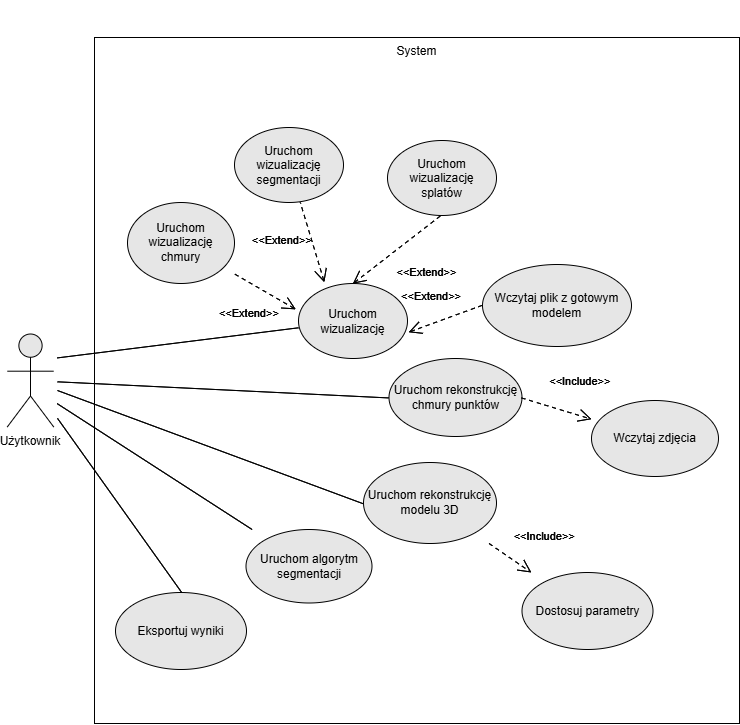
\includegraphics[width=1.0\linewidth]{img/diagramy/zpi use case.png}
    \caption{Diagram przypadków użycia}\label{fig:use_case_diagram}
  \end{figure}

\clearpage

\subsection{Architektura}

\begin{figure}[!htb]
    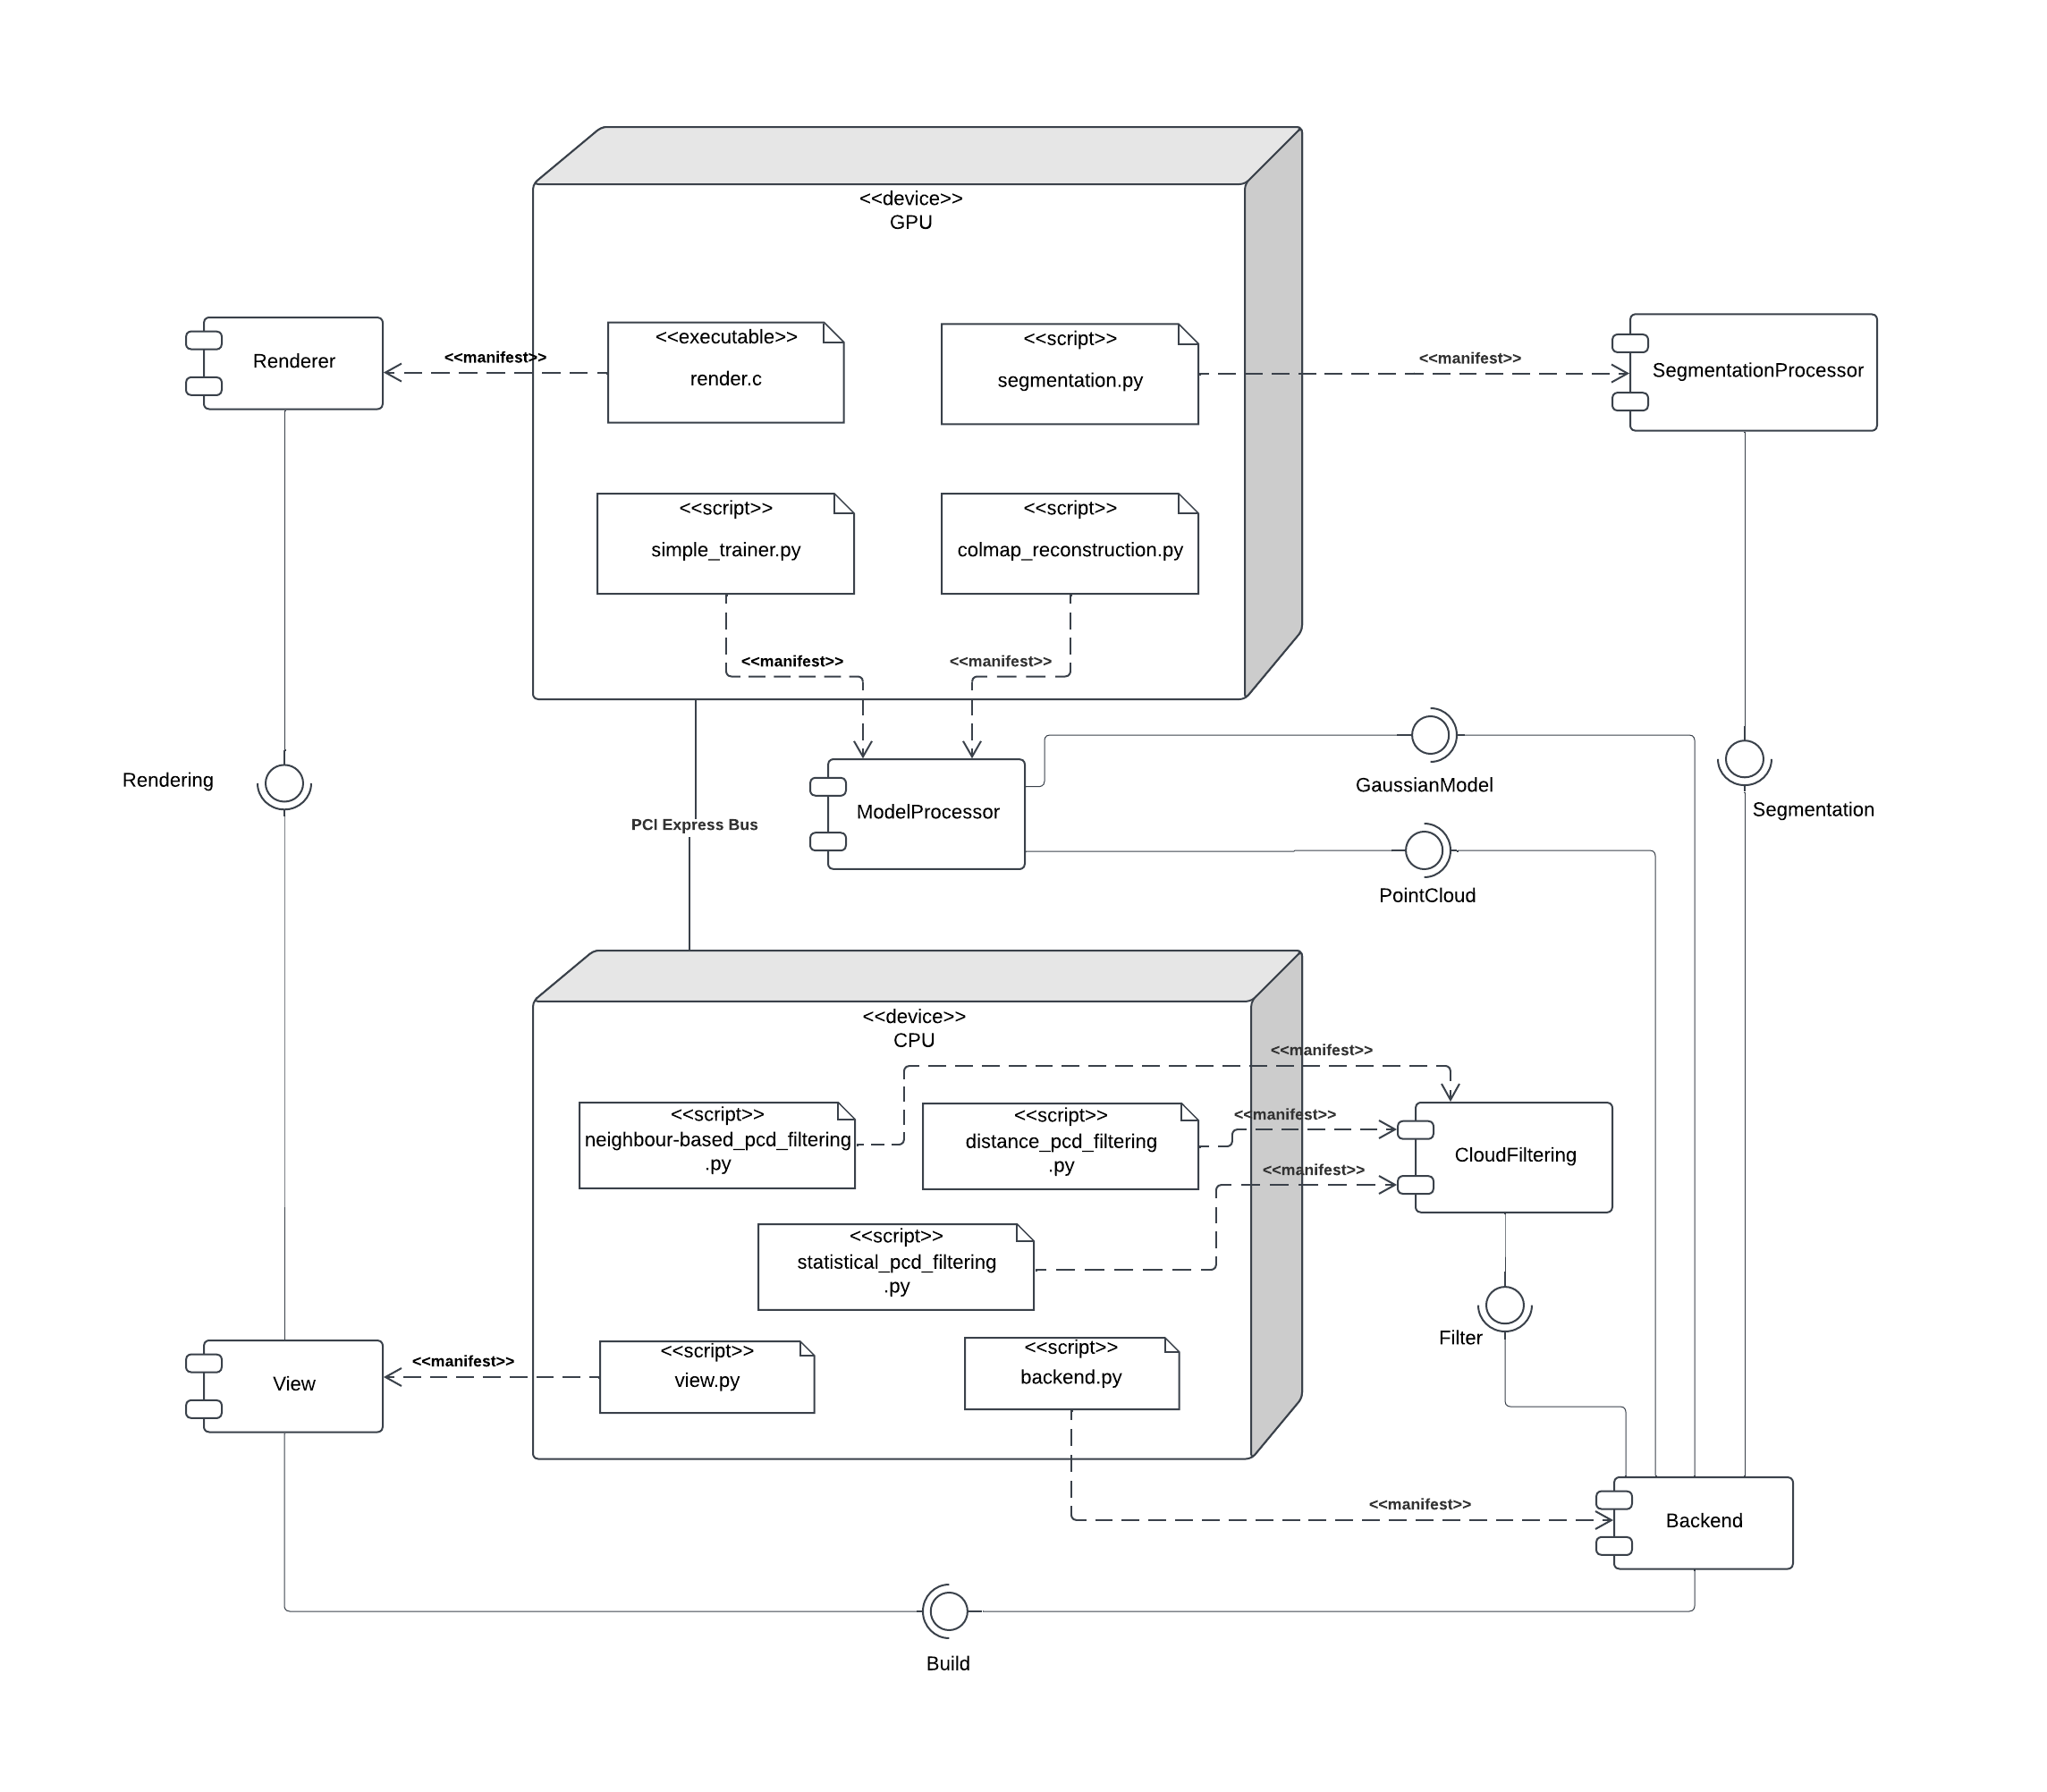
\includegraphics[width=1.0\linewidth]{img/diagramy/diagram_wdrozenia_komponentow_3.png}
    \caption{Diagram wdrożenia komponentów}\label{fig:components_diagram}
\end{figure}

\subsubsection{Architektura}
Projekt został zrealizowany w oparciu o wzorzec projektowy \textbf{MVVM} (Model-View-ViewModel), który został odpowiednio dostosowany do specyfiki aplikacji w celu zapewnienia modularności oraz uproszczenia procesu modyfikacji i rozbudowy.

\textbf{Adaptacja wzorca MVVM}
\begin{figure}[h!]
    \centering
    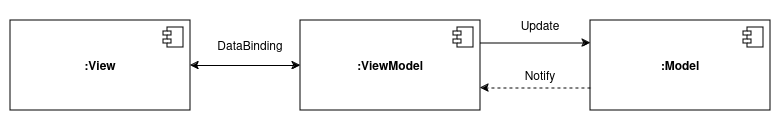
\includegraphics[width=0.8\textwidth]{img/diagramy/architektura.png}
    \caption{Schemat zaadaptowanego wzorca MVVM w projekcie.}
\end{figure}

W zaimplementowanym rozwiązaniu wzorzec \textbf{MVVM} został zmodyfikowany w celu optymalizacji komunikacji między komponentami aplikacji. Dzięki temu możliwe było osiągnięcie spójności architektury oraz jej wysokiej skalowalności.

\paragraph{Opis komponentów architektury}
\begin{figure}[h!]
    \centering
    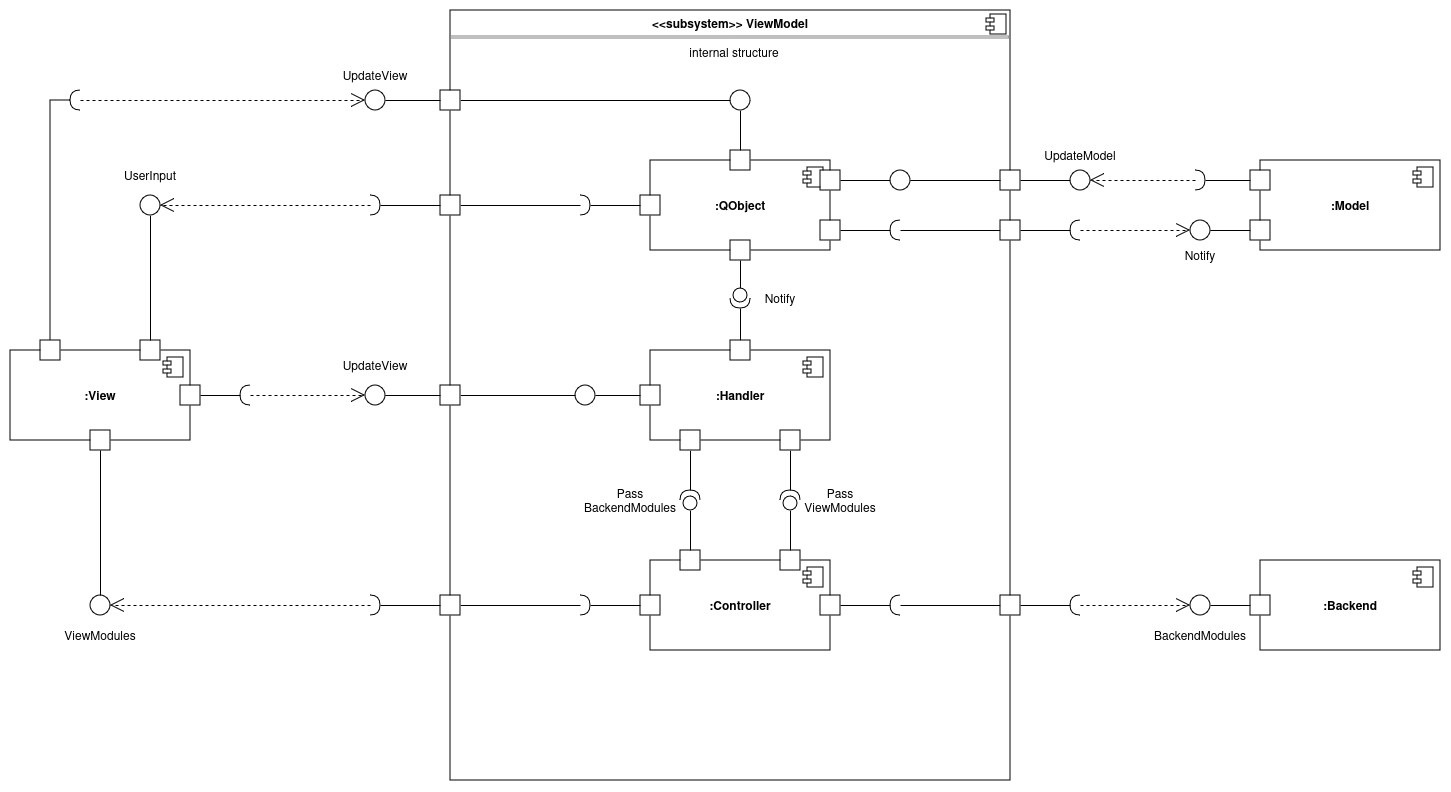
\includegraphics[width=0.8\textwidth]{img/diagramy/diagram_komp_vm.png}
    \caption{Struktura komponentów ViewModel w projekcie.}
\end{figure}

W projekcie klasa \texttt{ViewModel} zastępuje tradycyjny zbiór klas, takich jak:
\begin{itemize}
    \item \texttt{Controller} -- odpowiadający za sterowanie logiką,
    \item \texttt{QObject} -- obsługujący komunikację z frontendem,
    \item \texttt{Handler} -- integrujący dodatkowe funkcjonalności wizualne.
\end{itemize}

\textbf{Rola \texttt{QObject}}
Klasa \texttt{QObject} pełni funkcję tradycyjnego komponentu \texttt{ViewModel}, umożliwiając komunikację między warstwą logiki a frontendem aplikacji. Wykorzystuje mechanizm sygnałów dostarczany przez bibliotekę PyQt, co pozwala dynamicznie informować widok o zmianach stanu aplikacji.

\textbf{Handler jako rozszerzenie funkcjonalności}
\texttt{QObject} został wzbogacony o klasę \texttt{Handler}, która pozwala na łatwą implementację funkcji wizualnych w już istniejącej architekturze. Dzięki temu projekt zachowuje przejrzystość i elastyczność.

\textbf{Integracja za pomocą \texttt{Controller}}
Klasy \texttt{QObject} i \texttt{Handler} są zintegrowane za pomocą \texttt{Controller}, który zapewnia jednolity interfejs oraz ułatwia zarządzanie komponentami aplikacji.

Na diagramie widoczny jest dodatkowy komponent \textbf{Backend}, będący zbiorem skryptów, które dostarczają interfejs dla wymaganej funkcjonalności aplikacji. Backend odpowiada za obsługę logiki niezwiązanej bezpośrednio z widokiem oraz wspiera pozostałe komponenty architektury, zapewniając większą modularność.

\paragraph{Zalety wdrożonego rozwiązania}
Przedstawione rozwiązanie zapewnia następujące korzyści:
\begin{itemize}
    \item \textbf{Modularność} -- możliwość łatwego dodawania i modyfikowania komponentów bez ingerencji w istniejącą strukturę.
    \item \textbf{Skalowalność} -- umożliwia rozbudowę aplikacji o nowe funkcjonalności przy zachowaniu spójności architektury.
    \item \textbf{Wsparcie dla współbieżności} -- dzięki zastosowaniu mechanizmu sygnałów PyQt implementacja współbieżności jest intuicyjna i efektywna.
\end{itemize}

\paragraph{Podsumowanie}
Zaimplementowany wzorzec MVVM, w połączeniu z dodatkowymi modyfikacjami, pozwolił osiągnąć elastyczną i skalowalną architekturę aplikacji. Dzięki zastosowanemu podejściu projekt spełnia założenia modularności, umożliwiając łatwą rozbudowę oraz utrzymanie w przyszłości.

% \subsection{Implementacja}

\subsection{Wizualizacja}
W celu zapewnienia użytkownikowi końcowemu zintegrowanego i spójnego środowiska wizualizacji całego procesu – od wgrania plików wejściowych po interakcję z modelem – zaprojektowano od podstaw interfejs oraz system renderowania.

Założeniem projektu była implementacja intuicyjnego, dynamicznego i responsywnego \textbf{interfejsu}[\ref{fig:ui}] przy pomocy biblioteki \textit{PyQt} oraz języka \textit{QML}. Interfejs został zintegrowany z wydajnym systemem \textbf{renderingu}[\ref{fig:rendering}] GPU, wykorzystującym technologie \textit{OpenGL}, \textit{OpenCL} oraz język \textit{C}. Dodatkowo, użytkownik ma możliwość alternatywnego renderowania z wykorzystaniem biblioteki \textit{VisPy}.

Projekt rozwiązuje problem fragmentaryczności funkcji dostępnych w innych aplikacjach, oferując spójne środowisko do obsługi modeli 3D, obejmujące procesy tworzenia, modyfikacji, segmentacji oraz wizualizacji danych.
\\[10pt]
\textbf{Funkcjonalności interfejsu}

\begin{itemize} \item wybór zdjęć, \item ustawienie parametrów, \item generowanie chmury punktów, \item generowanie splatów, \item segmentacja splatów, \item wizualizacja wyników. \end{itemize}

\vspace{10pt}
{\setlength{\parindent}{0pt}
\textbf{Rendering}
}

Rendering wykorzystuje plik .ply jako dane wejściowe do wczytania splatów. Splaty te są reprezentowane przez sześciany z dodatkowymi parametrami przechowywanymi w Shader Storage Buffer Object (SSBO), co umożliwia efektywny odczyt dużych ilości danych. Takie podejście jest szczególnie przydatne w przypadku scen zawierających nawet do dwóch milionów obiektów.

Do przechowywanych parametrów należą: \begin{itemize} \item pozycja, \item skala, \item rotacja, \item kolor, \item przezroczystość. \end{itemize}

Podczas procesu renderowania, model sześcianu jest odpowiednio przekształcany na podstawie tych parametrów, co pozwala na uzyskanie splatów na wyjściu. Takie podejście umożliwia abstrakcyjne definiowanie splatów przy jednoczesnym zachowaniu wysokiej dokładności wizualnej.

\clearpage

\begin{figure}[!ht]
    \centering
    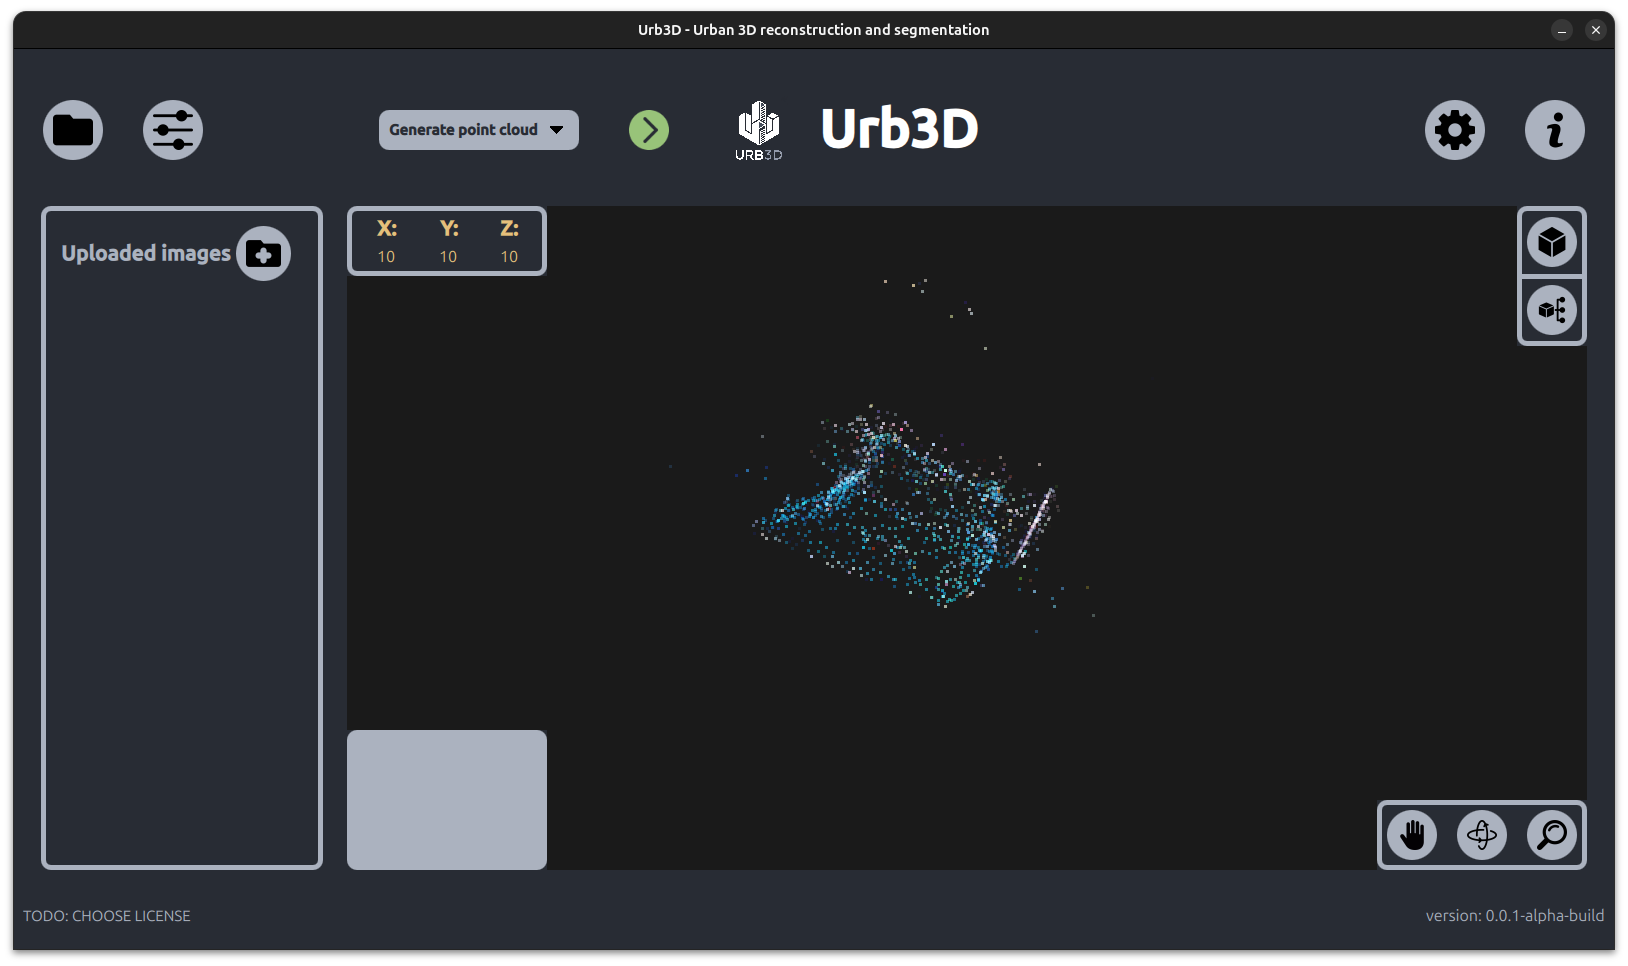
\includegraphics[width=\textwidth]{images/UI-Rendering.png}
    \caption{Zrzut ekranu przedstawiający główny widok aplikacji}
    \label{fig:ui}
\end{figure}

\begin{figure}[!ht]
    \centering
    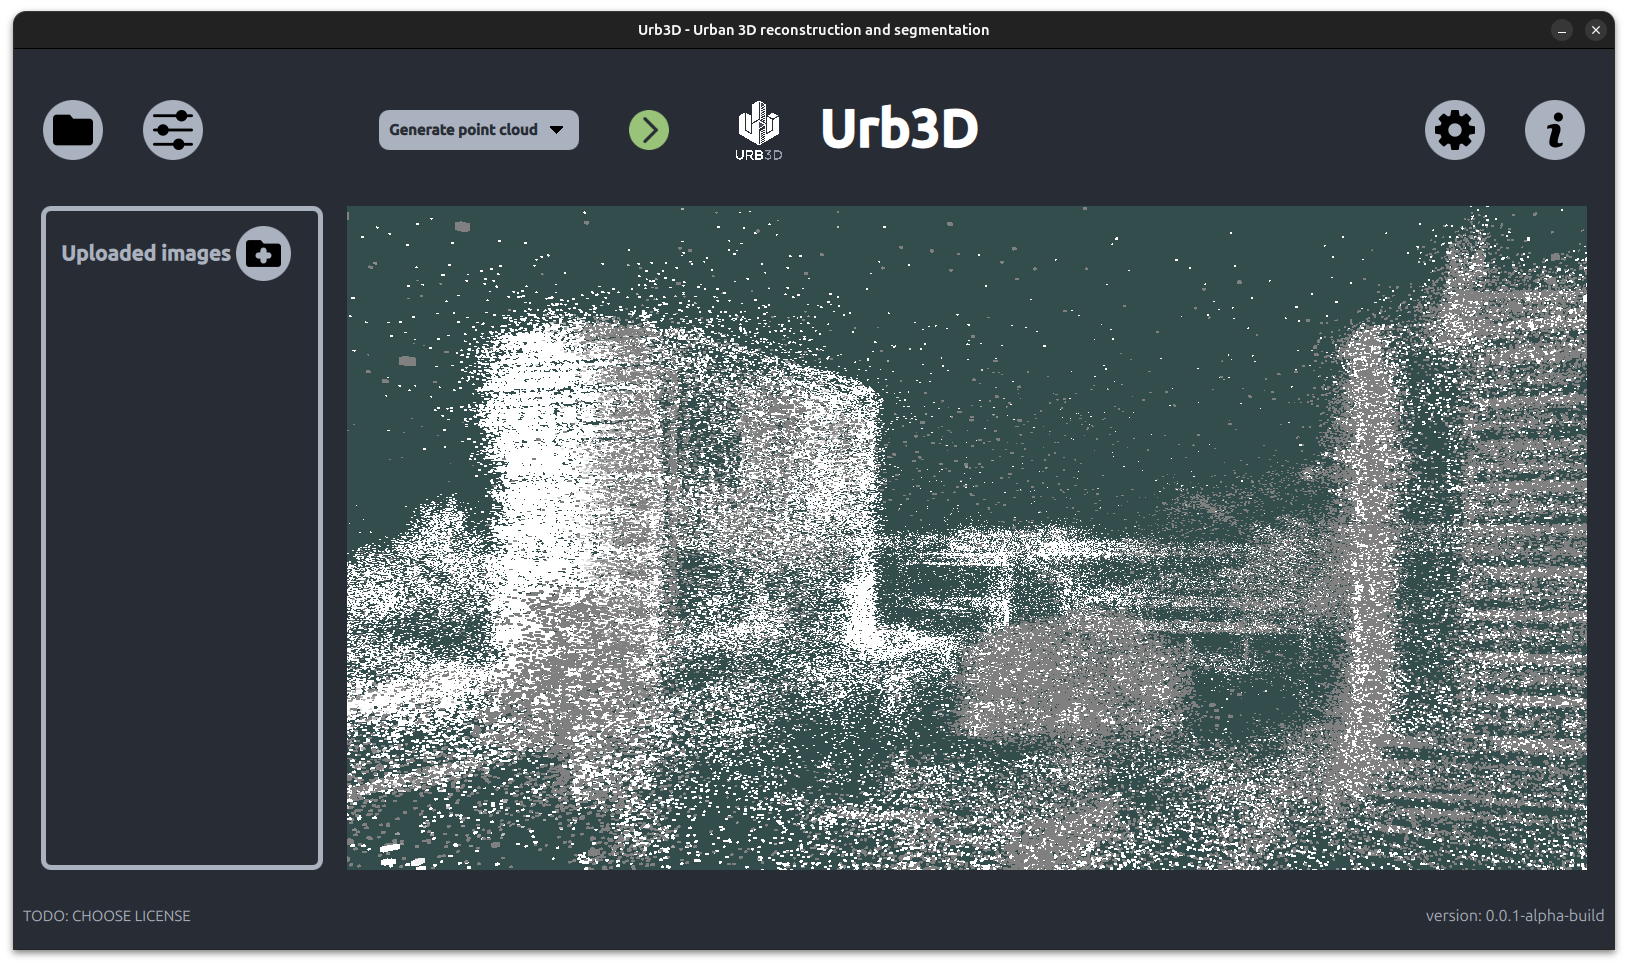
\includegraphics[width=\textwidth]{images/cloud_rendering.png}
    \caption{Zrzut ekranu przedstawiający własny renderer}
    \label{fig:rendering}
\end{figure}

\subsection{Rendering}

W aplikacji zaimplementowano autorski system renderingu w celu zapewnienia wysokiej wydajności oraz wygody użytkowania przez użytkownika końcowego. Do realizacji tego rozwiązania wykorzystano język C oraz bibliotekę OpenGL z rozszerzeniami GLEW, GLFW i CGLM.

\begin{figure}[h!]
    \centering
    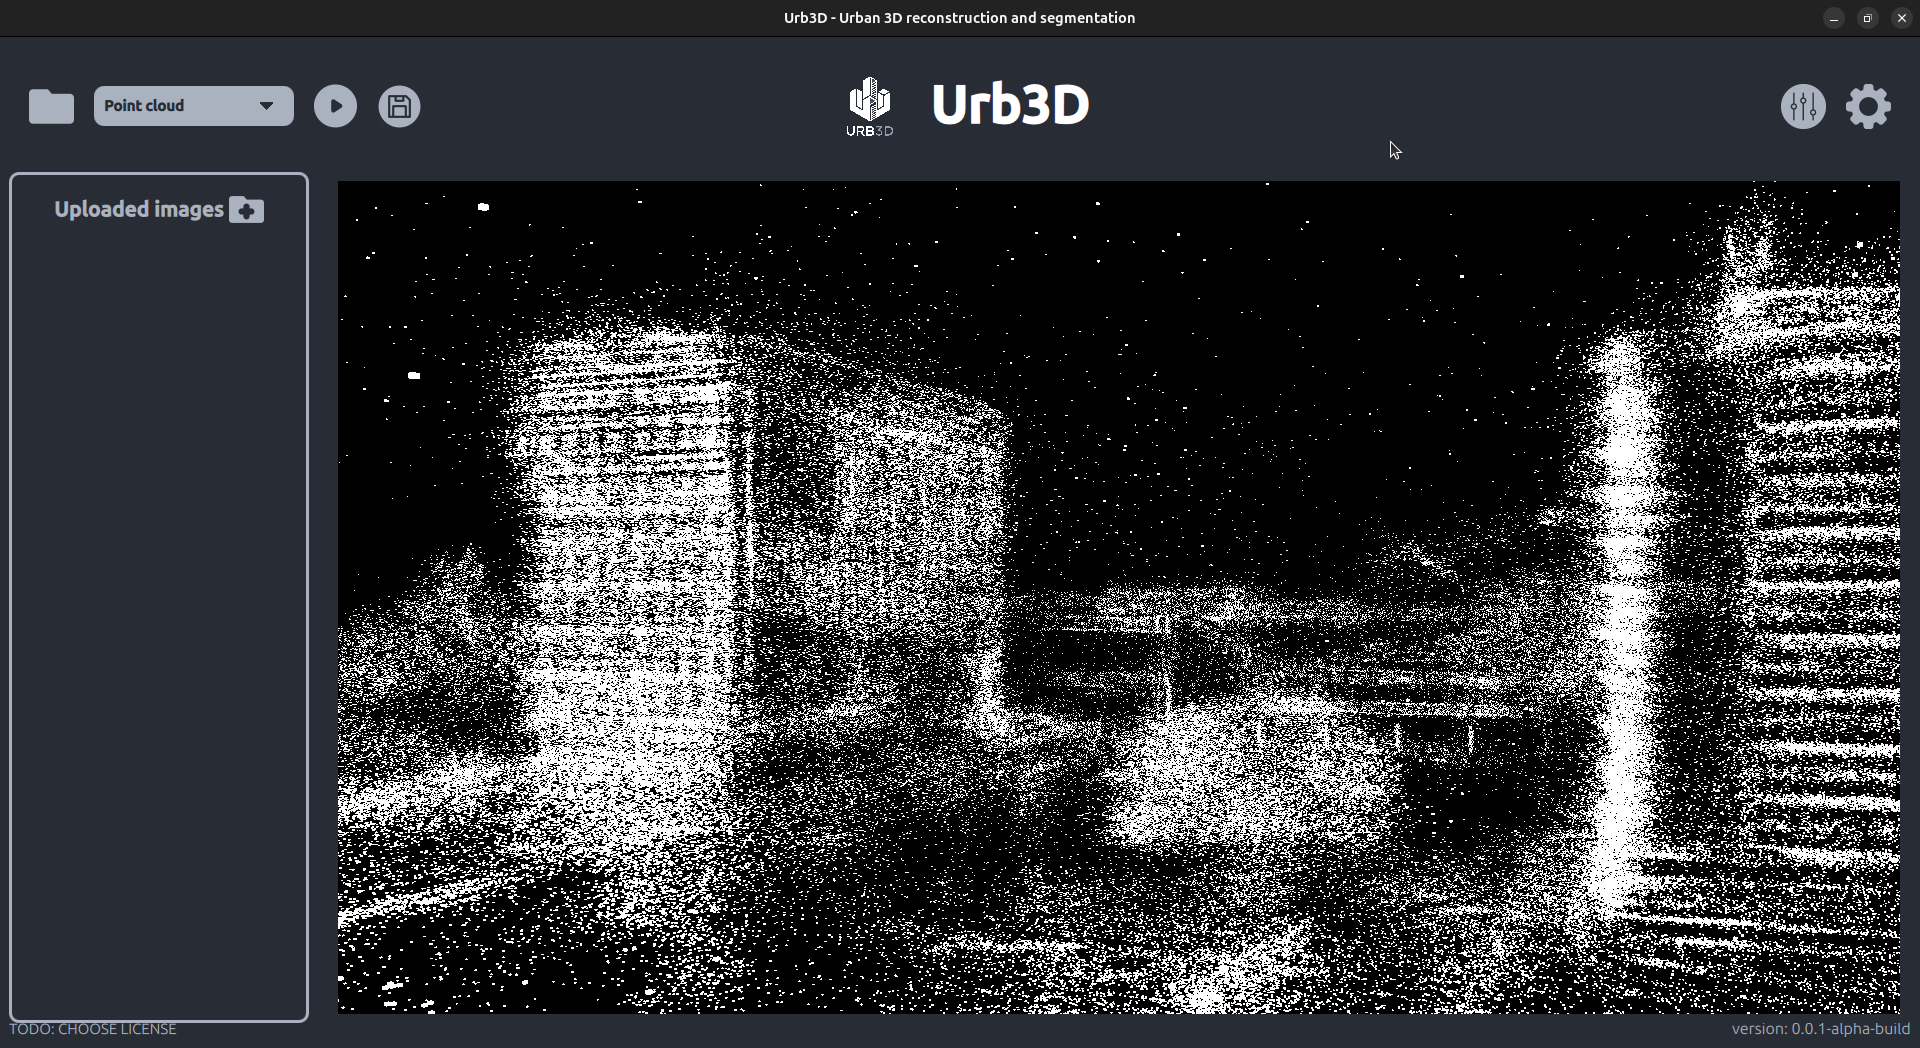
\includegraphics[width=0.8\textwidth]{img/wizualizacja/ui_rendering.png}
    \caption{Widok główny aplikacji z zaimplementowanym renderingiem.}
    \label{fig:widok_glowny}
\end{figure}

\subsubsection{Integracja z Pythonem}
Rendering został udostępniony jako dynamiczna biblioteka współdzielona, co umożliwia jego integrację z aplikacjami napisanymi w języku Python. Dzięki temu, w połączeniu z frameworkiem PyQt, rendering może być efektywnie wykorzystywany w aplikacjach graficznych.

\begin{figure}[h!]
    \centering
    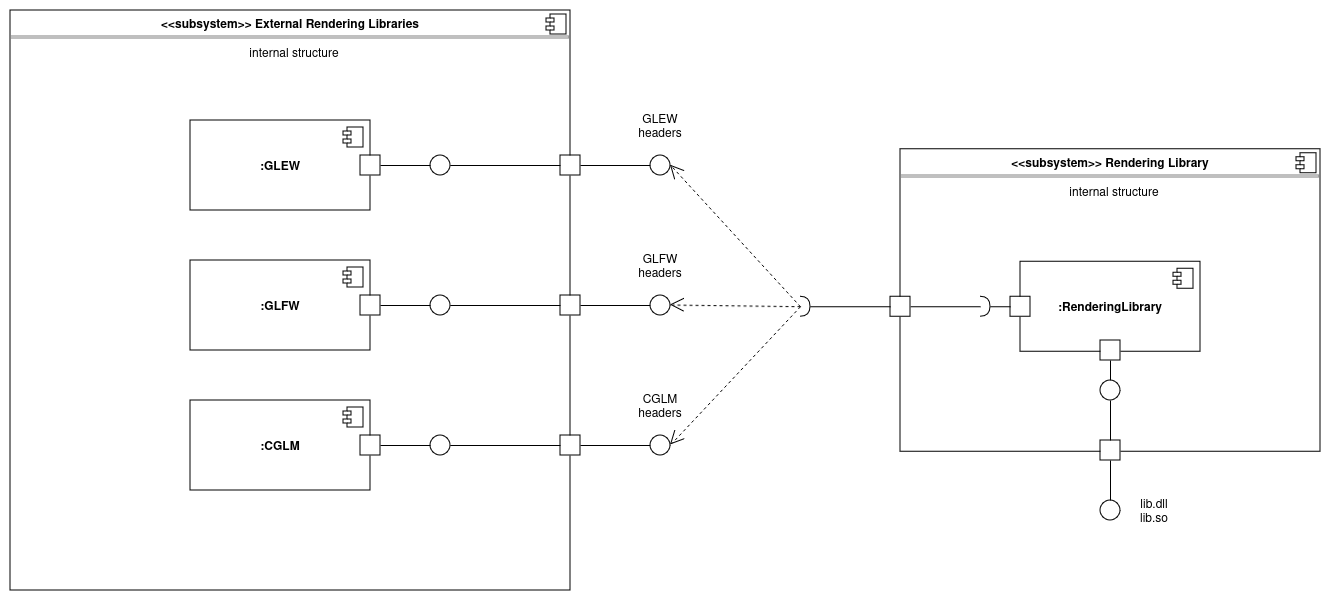
\includegraphics[width=0.8\textwidth]{img/diagramy/diagram_komp_rendering.png}
    \caption{Diagram przedstawiający architekturę integracji renderingu z Pythonem.}
    \label{fig:diagram}
\end{figure}

\subsubsection{Implementacja systemu renderingu}

\textbf{Reprezentacja punktów i splatów}
Wizualizacja punktów oraz splatów została zrealizowana za pomocą sześcianów, które są skalowane i rotowane w taki sposób, aby przypominały elipsoidy. Przetworzone w ten sposób sześciany są następnie renderowane przy użyciu shaderów, co pozwala na uzyskanie efektu ich zaokrąglenia.

\textbf{Optymalizacja wydajności}
Aby zwiększyć wydajność obliczeń graficznych, wykorzystano GPU z użyciem obiektów SSBO (Shader Storage Buffer Objects). SSBO umożliwiają przechowywanie i przetwarzanie dużych ilości danych bezpośrednio na karcie graficznej, co minimalizuje obciążenie procesora głównego.

\clearpage

W ramach procesu renderingu wczytywane są dane statyczne dla domyślnego sześcianu, a następnie przetwarzane są atrybuty poszczególnych punktów, takie jak:
\begin{itemize}
    \item pozycja,
    \item skalowanie,
    \item rotacja,
    \item przezroczystość,
    \item kolor.
\end{itemize}

Takie podejście zapewnia elastyczność oraz wysoką wydajność w generowaniu scen 3D.

% \clearpage

\subsection{Technologie}

W projekcie wykorzystano następujące technologie

\begin{itemize}
    \item \textbf{C/C++}: OpenCL, OpenGL
    \item \textbf{Python}: Pytorch, pycolmap, open3d, pyvista, PyQt (numpy, matplotlib), pytest
    \item CloudCompare, Meshlab
    \item \textbf{GPU}
    \item Jira, Confluence, Github, Discord
\end{itemize}

\begin{figure}[!ht]
    \centering
    
\includegraphics[width=0.9\linewidth]{img/sota/technologie.png}
  \end{figure}

\subsubsection{Struktura plikowa projektu}

% millon opcji https://tex.stackexchange.com/questions/5073/making-a-simple-directory-tree
\begin{forest}
  for tree={
    grow'=0,
    child anchor=west,
    parent anchor=south,
    anchor=west,
    calign=first,
    edge path={
      \noexpand\path [draw, \forestoption{edge}] (!u.south west) ++(3pt,0) -- +(-3pt,0) |- (.child anchor)\forestoption{edge label};
    },
    before typesetting nodes={
      if n=1
        {insert before={[,phantom]}}
        {}
    },
    fit=band,
    before computing xy={l=15pt},
  }
[project
  [data
    [city\_model
      [images]
      [sparse
          [images.bin]
          [cameras.bin]
          [points.bin]
          [sparse.ply]
      ]
      [filtered\_model.ply]
      [model.pt]
      [model.ply]
      [model\_seg.ply]
    ]
    [pointnet-ckpt.pt]
  ]
  [scripts]
  [src
    [frontend]
    [backend]
    [urb3d
      [datasets]
      [pipeline]
      [segmentation]
      [rendering]
      [geometry]
      [models]
      [splats]
    ]
  ]
  [test]
]
\end{forest}

\subsection{Akwizycja danych}
W projekcie założono wykorzystanie metod fotogrametrycznych do tworzenia trójwymiarowych modeli 
obszarów urbanistycznych. Za część projektu przyjęto z tego względu również pozyskanie własnych zestawów 
danych fotograficznych (fotogramów), które spełniałyby wymogi techniczne, umożliwiające późniejszą 
rekonstrukcję 3D. Niezbędne było wykonanie dużej liczby ujęć, obejmujących wiele kątów i perspektyw oraz 
zapewnienie odpowiedniego nakładania się zdjęć dla poprawnego działania oprogramowania fotogrametrycznego, 
które identyfikuje i dopasowuje wspólne punkty widoczne na wielu zdjęciach.

Akwizycję zrealizowano na kampusie \textbf{Politechniki Wrocławskiej}, koncentrując się na budynkach \textbf{C5}, \textbf{C7} oraz 
Strefie Kultury Studenckiej (\textbf{SKS}) \ref{fig:four-photos} i pozyskując zdjęcia zarówno z lotów bezzałogowym statkiem powietrznym, 
jak i z poziomu gruntu. Stanowią one kompletne zbiory danych, które spełniły wymogi jakościowe 
i posłużyły do budowy testowych modeli. 

\begin{figure}[h!]
    \centering
    \begin{minipage}{0.245\textwidth}
        \centering
        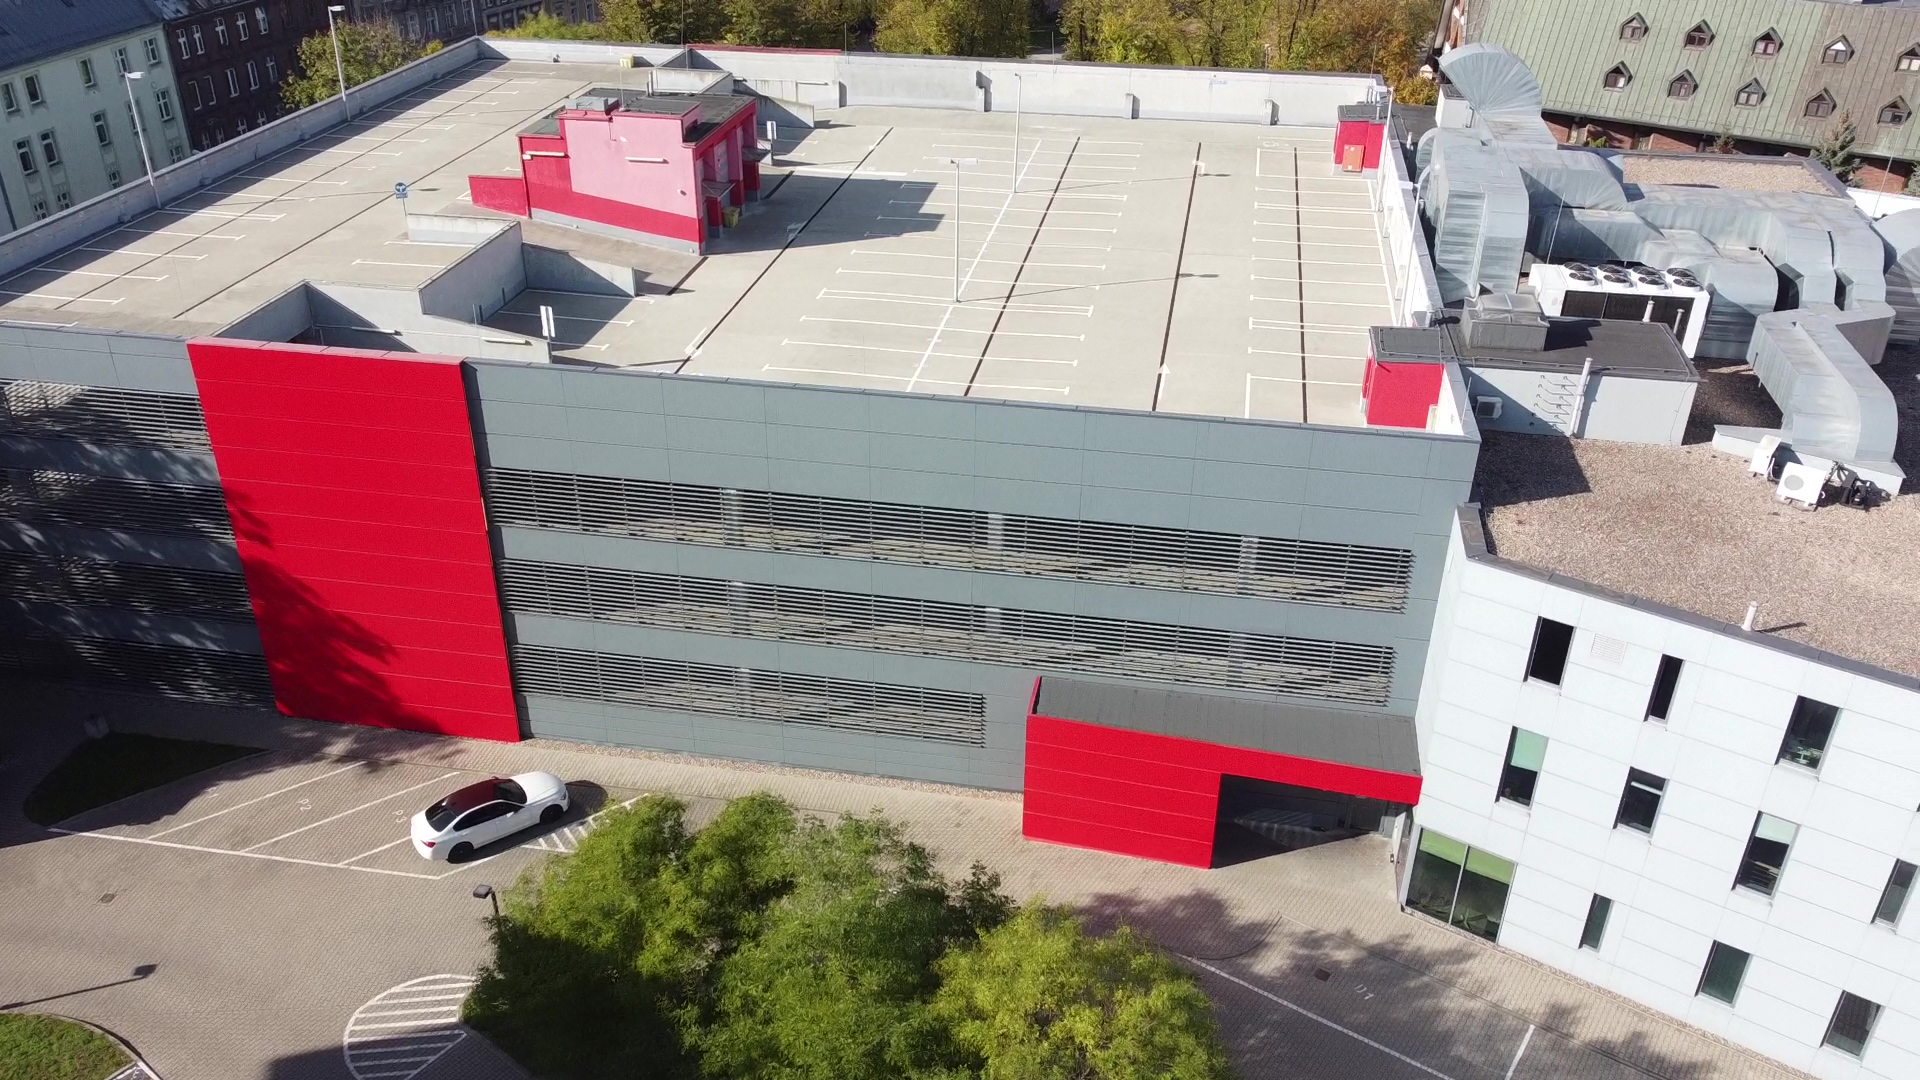
\includegraphics[width=\textwidth]{images/sks_dataset_1.jpg}
    \end{minipage}
    \hfill
    \begin{minipage}{0.245\textwidth}
        \centering
        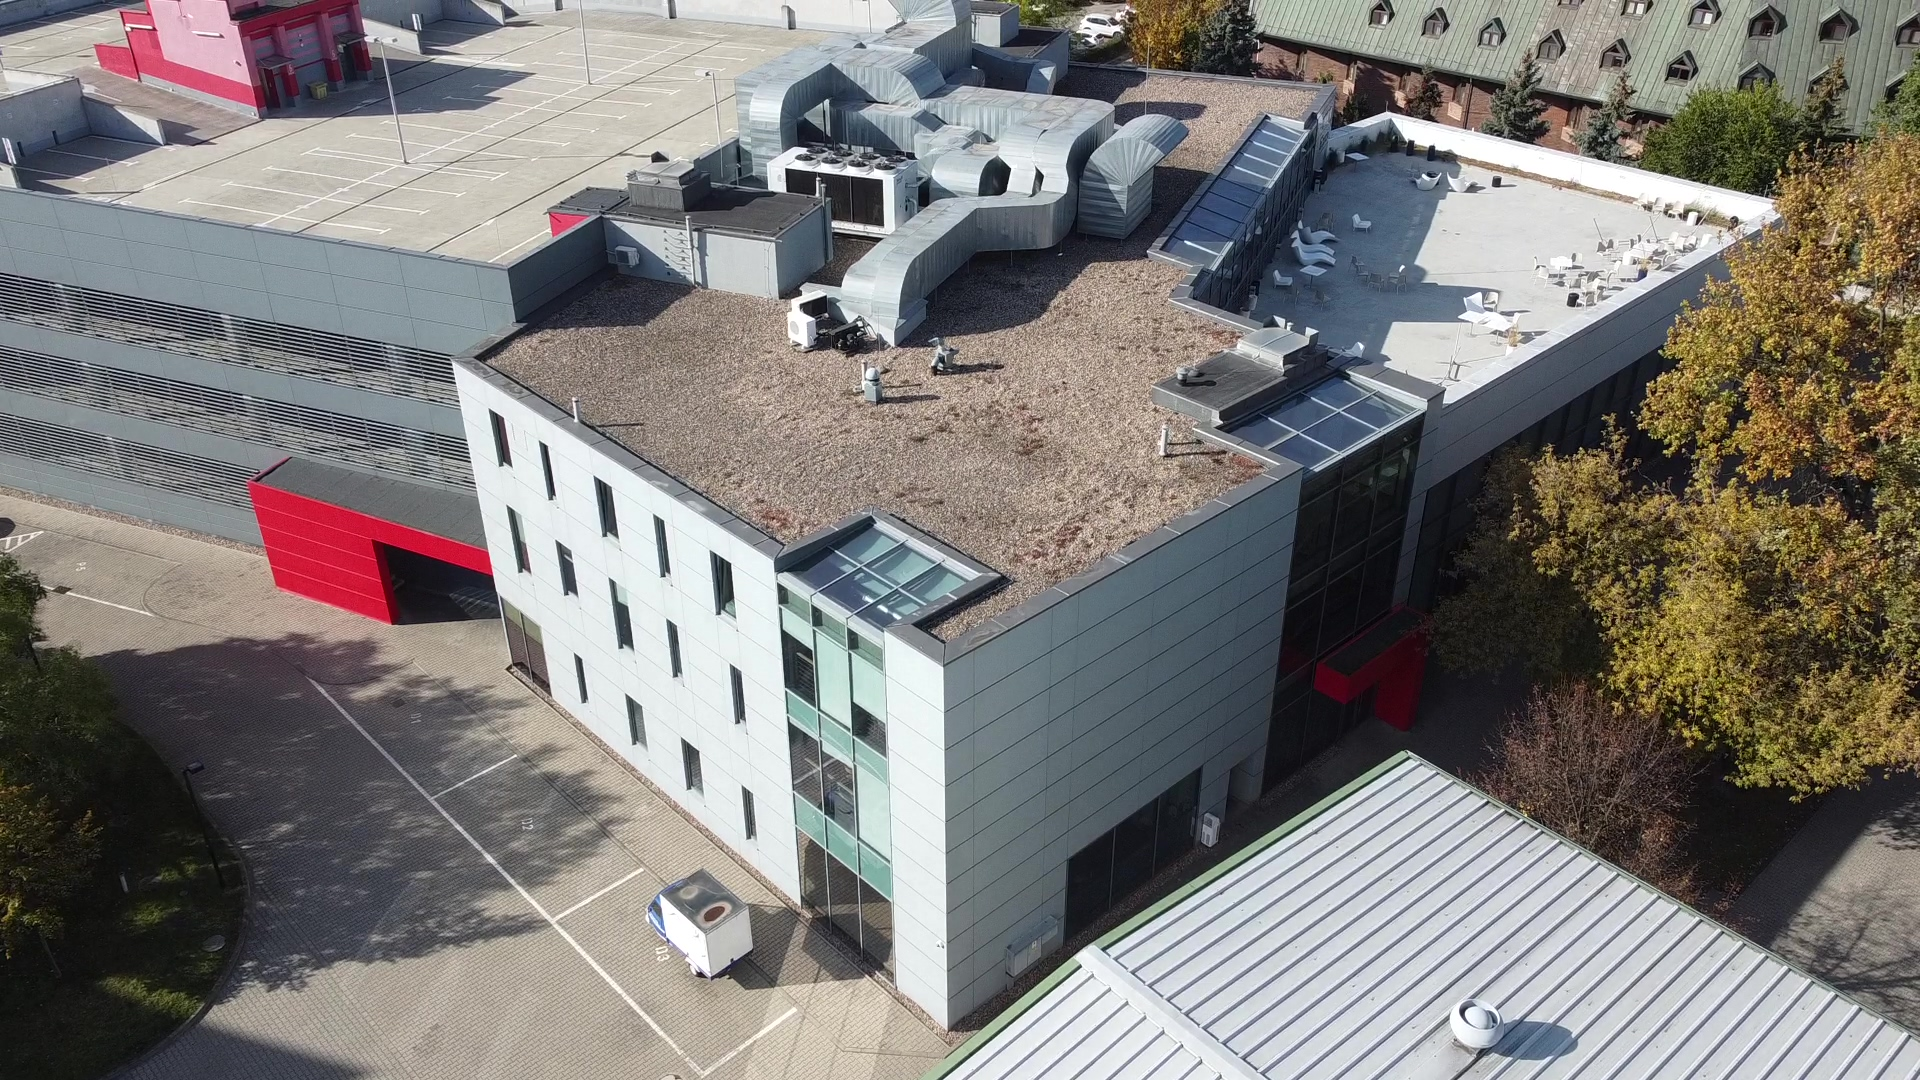
\includegraphics[width=\textwidth]{images/sks_dataset_2.jpg}
    \end{minipage}
    \hfill
    \begin{minipage}{0.245\textwidth}
        \centering
        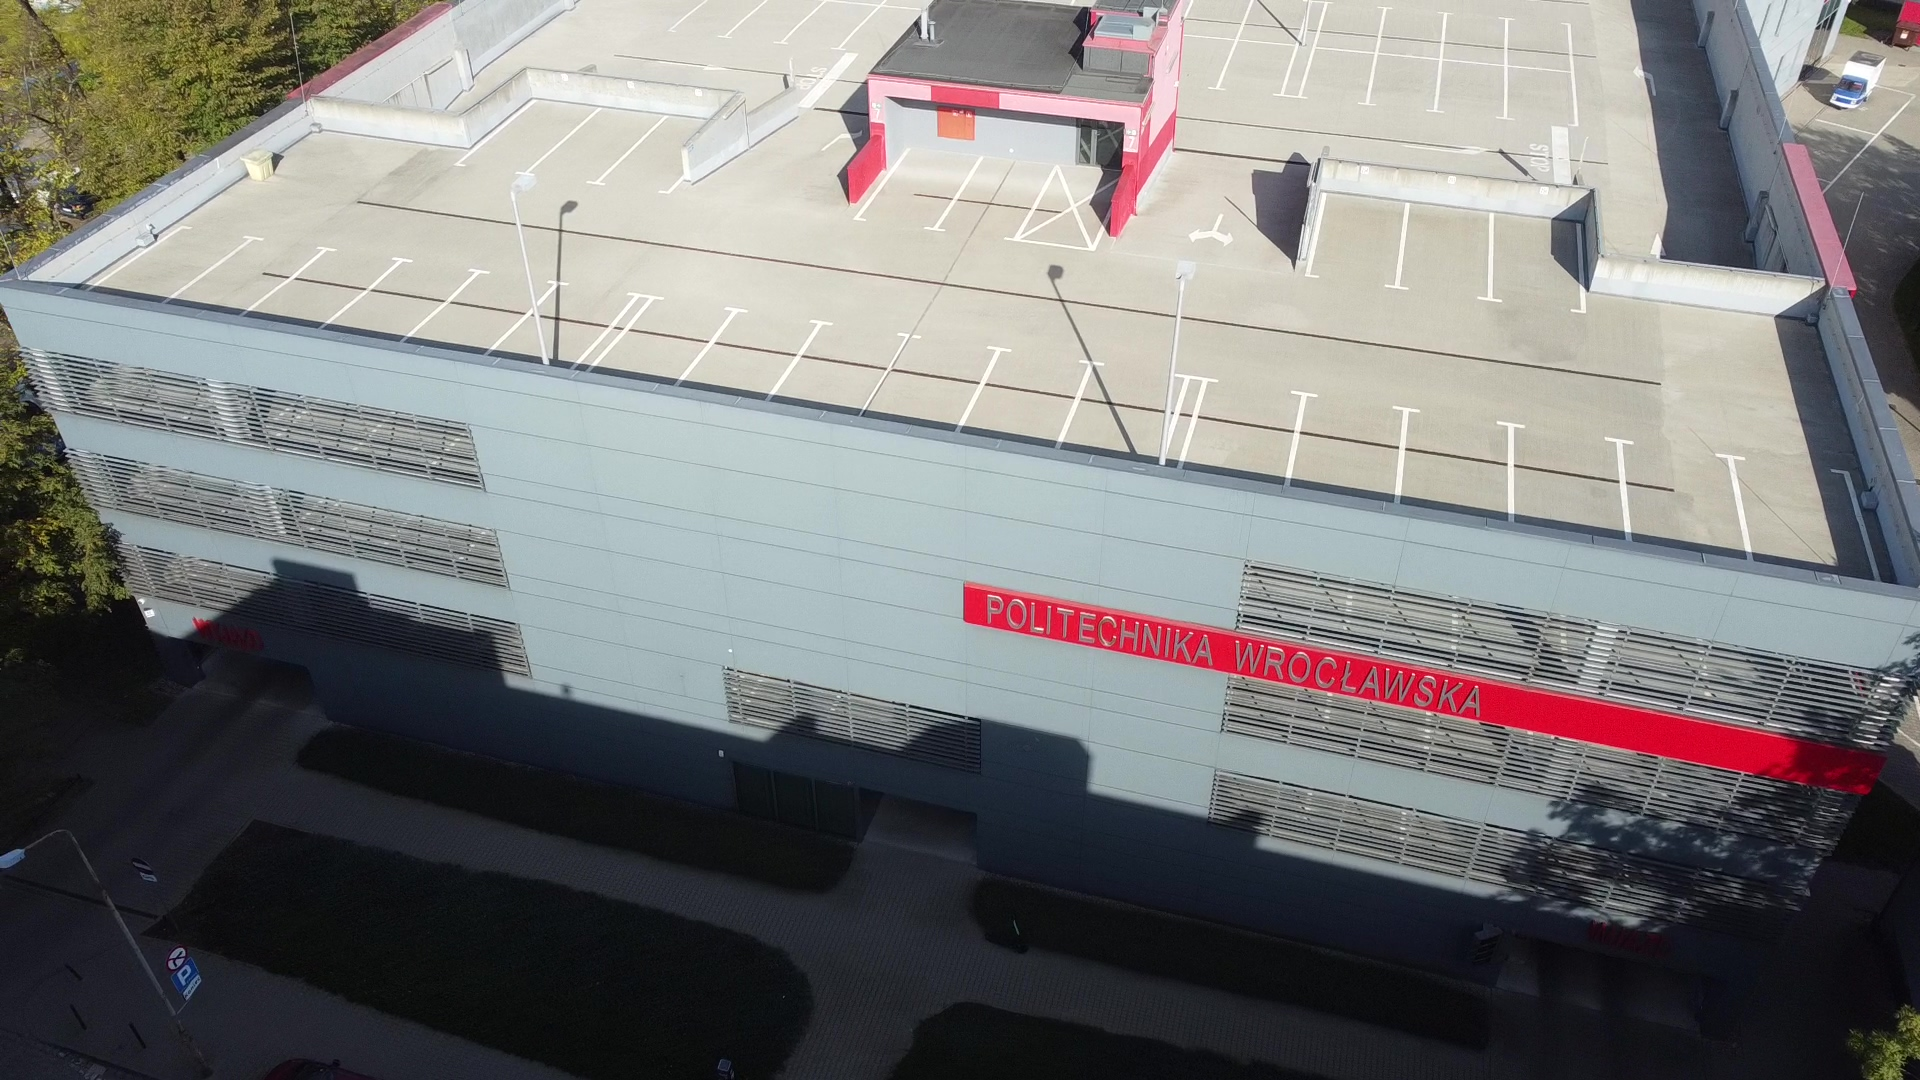
\includegraphics[width=\textwidth]{images/sks_dataset_3.jpg}
    \end{minipage}
    \hfill
    \begin{minipage}{0.245\textwidth}
        \centering
        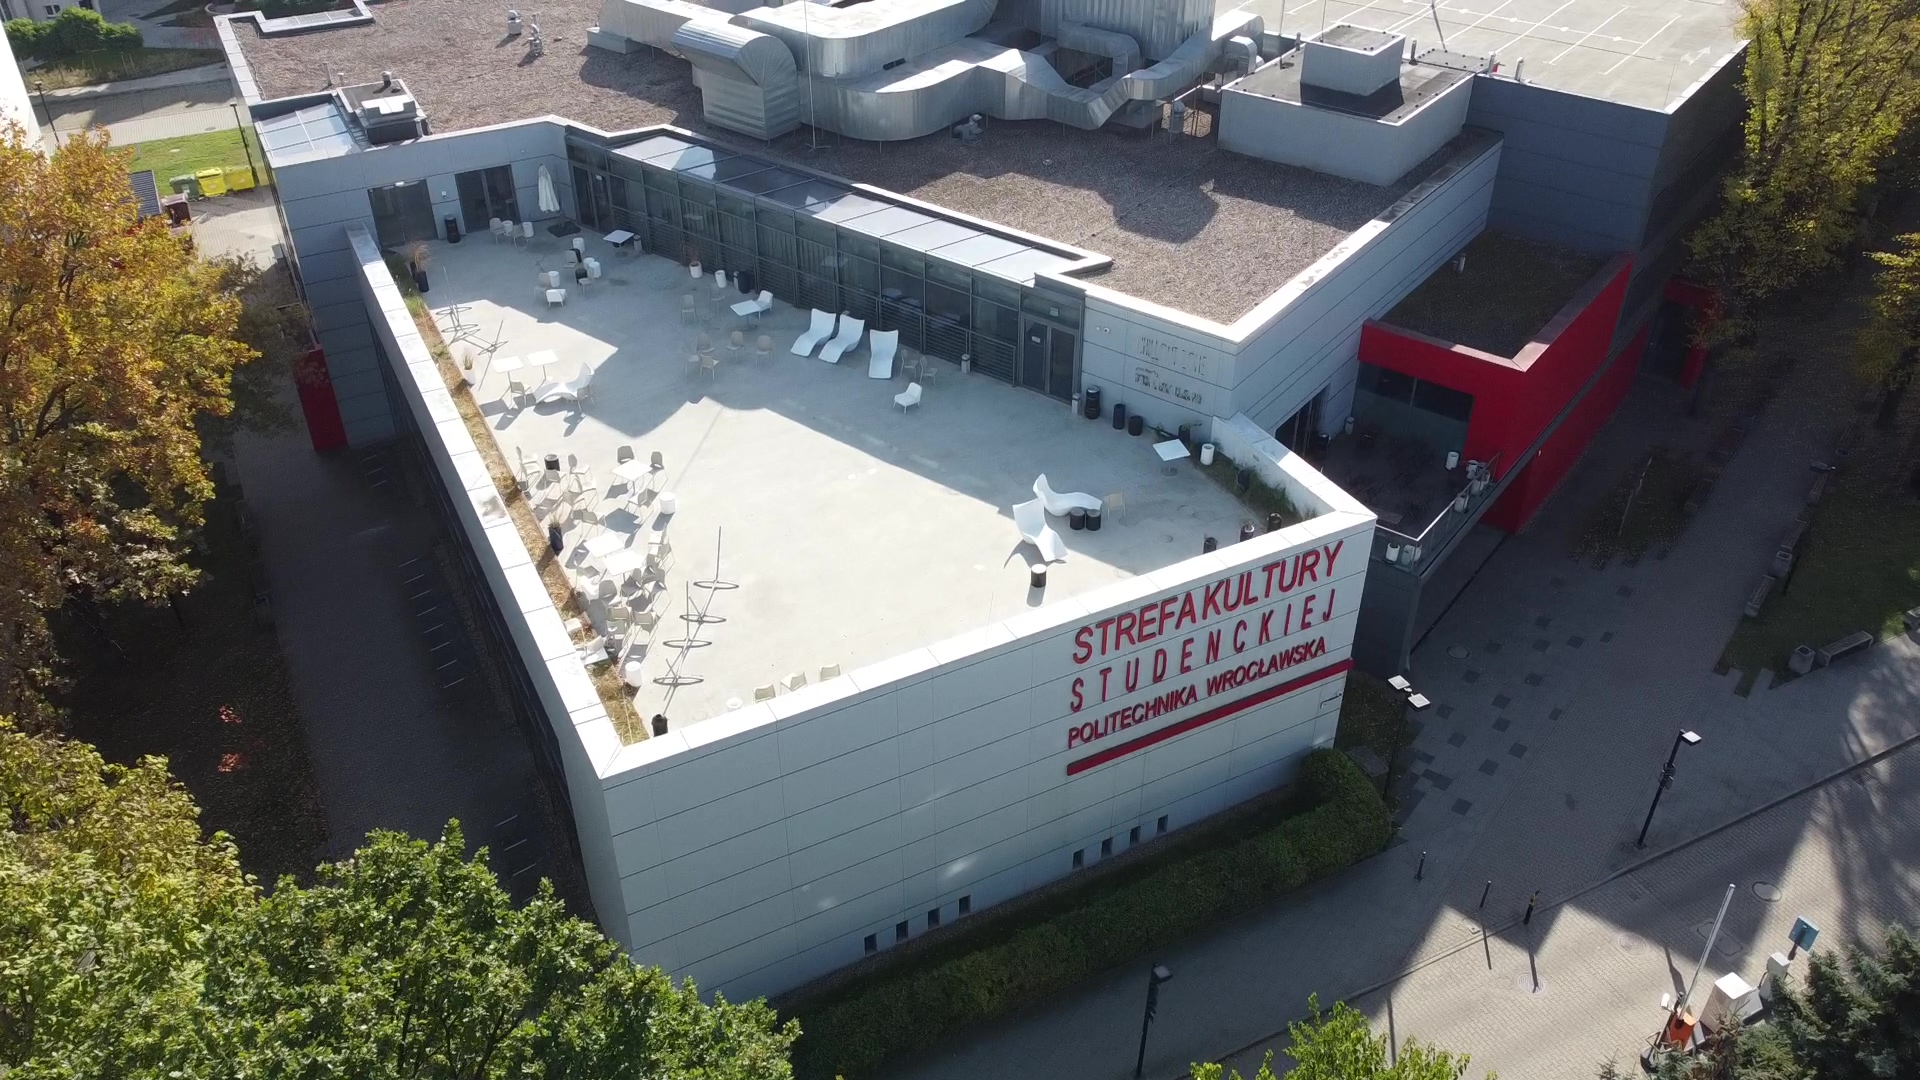
\includegraphics[width=\textwidth]{images/sks_dataset_4.jpg}
    \end{minipage}
    \caption{Przykładowe zdjęcia z akwizycji danych przedstawiające SKS}
    \label{fig:four-photos}
\end{figure}

\subsection{Structure from motion}
Kolejnym etapem projektu było wykorzystanie techniki \textit{Structure from Motion} (SfM) do wyznaczania
struktur przestrzennych scen na podstawie dobranych zestawów zdjęć dwuwymiarowych. 

Algorytmy SfM, identyfikując i łącząc 
punkty wspólne między zdjęciami, ustalają zarówno rozmieszczenie tych punktów w przestrzeni, jak i pozycje 
i orientacje kamer, z których wykonano zdjęcia. Proces ten pozwala na oszacowanie struktury trójwymiarowej
sfotografowanego obszaru, czyli wygenerowanie chmury punktów odwzorowującej scenę w postaci 
zbioru punktów 3D o przypisanych kolorach, tak jak to pokazano na \ref{fig:example_recon}. 

Do realizacji tego zadania użyliśmy popularnego narzędzia COLMAP, a konkretnie jego wersji w formie biblioteki 
\textit{pycolmap}, oferującej funkcjonalności m.in. do wykrywania charakterystycznych cech na obrazach, 
łączenia punktów wspólnych na zdjęciach czy przeprowadzania rekonstrukcji sceny 3D na podstawie dopasowań 
między nimi.

Uzyskana w ten sposób trójwymiarowa reprezentacja sceny w postaci chmury punktów służy za podstawę do 
modelowania z zastosowaniem algorytmu Gaussian Splatting. 

\begin{figure}[!ht]
    \centering
    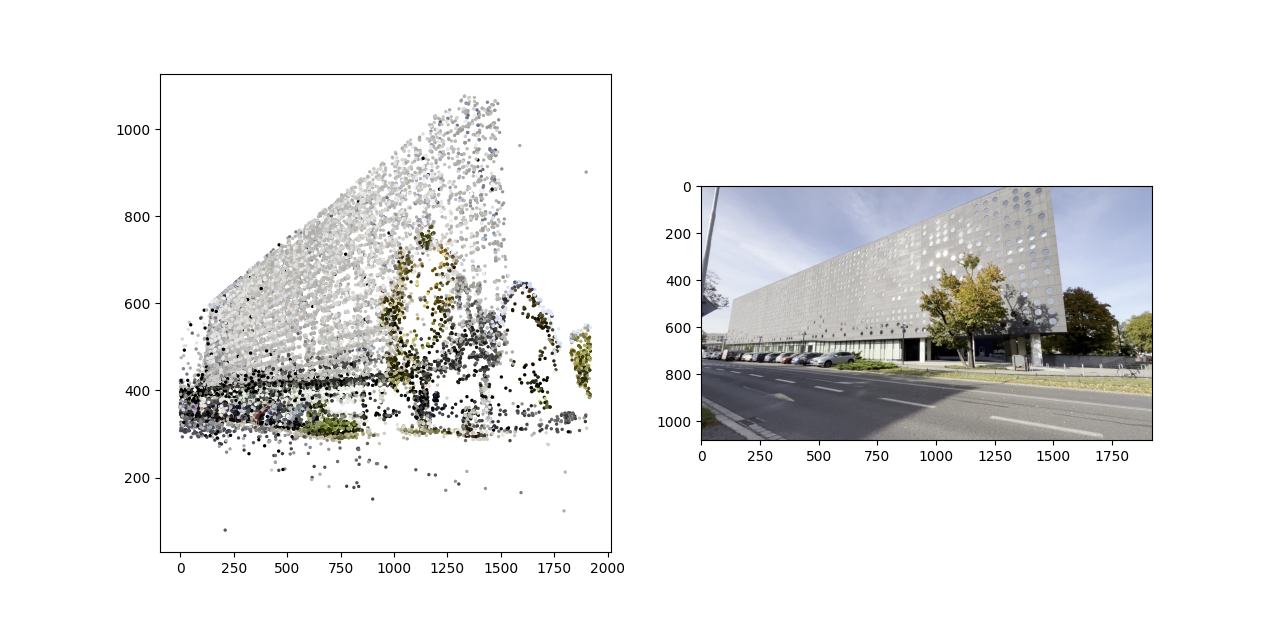
\includegraphics[width=0.9\linewidth]{images/sfm.png}
    \caption{Projekcja przykładowej chmury punktów na płaszczyznę porównana do zdjęcia}
    \label{fig:example_recon}
\end{figure}

\subsection{Gaussian Splatting}
Przy pomocy biblioteki \textit{gsplat}\cite{ye2024gsplatopensourcelibrarygaussian} zawierającej implementację \textit{Gaussian Splatting} w Pythonie wykonaliśmy eksperymenty polegające na uruchomeniu algorytmu dla różnych wartości hiperparametrów w celu znalezienia wartości, które prowadzą do jak najbardziej optymalnego procesu trenowania w kontekście czasu trwania i wykorzystania pamięci. 

Na wejściu algorytmu podawana jest otrzymywana w procesie rekonstrukcji chmura punktów, która jest bazą do dalszego dzielenia i powstawania "gaussianów", a ich parametry: pozycja, kolor, skala i rotacja są optymalizowane przy pomocy metody spadku wzdłuż gradientu. Metryki przyjęte do oceny jakości to SSIM (Structural Similarity Index Measure), PSNR (Peak Signal-to-Noise Ratio) oraz LPIPS (Learned Perceptual Image Patch Similarity).

W wyniku przeprowadzenia eksperymentów okazało się, że najważniejszymi sterującymi procesem parametrami są 
\begin{enumerate}
    \item Liczba Gaussianów: w przypadku scen urbanistycznych w celu oddania odpowieniej szczegółowości potrzebne jest parę milionów Gaussianów, dla naszych scen było to zwykle 3 mln.
    \item Strategia i częstość adaptacji: określają w jaki sposób oraz jak często dodawane i usuwane są Gaussiany. 
    \item Liczba iteracji: zwykle im dłużej trenowana jest scena tym lepsze wyniki otrzymujemy, jednak zależy to również od przyjętej strategii. Liczba ta wpływa bezpośrednio na czas trenowania, powinna wynieść nie mniej niż paręnaście tysięcy.
    \item Stopień zmiennych harmonicznych: wyrażają one kolor, im większy stopień tym lepsza jakość sceny, ale też zwiększone zużycie pamięci i wydłużony czas trenowania. 
\end{enumerate}

Poniżej przedstawione są przykładowe wizualizacje. Renderowania zostały wykonane przy pomocy biblioteki nerfview która również służy do wizualizacji splatów. Na poniższych rysunkach są od lewej do prawej: prawdziwe zdjęcie i widok modelu.

\begin{figure}[!h]
    \centering
    \includegraphics[width=1.0\linewidth]{images/sks_viper_0008.png}
    \caption{Scena SKS}
    \label{fig:sks_gs}
\end{figure}

\begin{figure}[!h]
    \centering
    \includegraphics[width=1.0\linewidth]{images/c5_mouse_0001.png}
    \caption{Scena C5}
    \label{fig:c5_gs}
\end{figure}

\begin{figure}[!h]
    \centering
    \includegraphics[width=1.0\linewidth]{images/c7_gepard_0006.png}
    \caption{Scena C7}
    \label{fig:c7_gs}
\end{figure}

\begin{table}[!h]
    \centering
    \begin{tabular}{|c|c|c|c|c|}
    \hline
    scena & PSNR & SSIM & LPIPS & liczba gaussianów \\
    \hline 
    SKS & 22.03 & 0.71 & 0.25 & 2,937,549 \\
    \hline 
    C5 & 0.0 & 0.0 & 0.0 & 0.0 \\
    \hline 
    C7 & 22.63 & 0.72 & 0.29 & 3,000,000 \\
    \hline
    \end{tabular}
\caption{Całościowe metryki dla testowych scen}
\label{table:tab_conf_sks}
\end{table}

\subsection{Segmentacja semantyczna}
Otrzymana w wyniku poprzednich etapów chmura punktów poddawana procesowi segmentacji semantycznej, czyli przypisaniu każdemu z punktów odpowiedniej kategorii semantycznej opisującej obiekt, w skład którego wchodzi. Do wybranych (na podstawie popularnych w literaturze zbiorów danych służących za punkt odniesienia w testowaniu modeli) kategorii semantycznych należą między innymi \textit{budynek}, \textit{droga}, czy też \textit{zieleń miejska}. 
Używając biblioteki \textit{PyTorch} do uczenia głębokiego, w oparciu o istniejące rozwiązania i aktualny stan wiedzy, przygotowano i wytrenowano własne modele \emph{sieci neuronowych} do segmentacji semantycznej.
W procesie eksperymentowania z różnymi architekturami i sposobami implementacji procesu treningu i predykcji za kluczowe pod względem wpływu na osiągi otrzymanego modelu należy uznać:
\begin{enumerate}
    \item próbkowanie - przy przetwarzaniu zbiorów danych, w przypadku których określenie porządku jest z punktu widzenia efektywności rozwiązania bezcelowe, a które jednocześnie z punktu widzenia modelu mogą osiągać różne rozmiary, ważnym elementem procesu zarówno treningu, jak i predykcji jest odpowiednie próbkowanie całego zbioru. Jest to niezbędne ze względu na architekturę sieci neuronowych, która zakłada stały rozmiar wejścia do modelu. W obrębie tego problemu należy wyróżnić następujące czynniki:
    \begin{enumerate}
        \item rozmiar próbki - zbyt mały może uniemożliwić uchwycenie zależności pomiędzy zbliżonymi do siebie w chmurze punktami,
        \item sposób próbkowania - wpływa na zależność uchwyconych w wyniku procesu uczenia wzorców od bardziej lub mniej odległych od siebie punktów. Może prowadzić do swego rodzaju zdominowania segmentowanych punktów przez jedną kategorię.
    \end{enumerate}
    \item niezbalansowany zbiór danych - w przypadku rozpatrywania dużych scen miejskich naturalnym jest pojawienie się mniej (\textit{samochody}, \textit{tory kolejowe}) i bardziej (\textit{budynki}) popularnych kategorii semantycznych. Jest to klasyczny problem uczenia maszynowego na niezbalansowanym zbiorze danych, który, niezaadresowany, prowadzi do dominacji zbioru przez punkty popularniejszych kategorii, w efekcie przekładając się na słabszą generalizację otrzymanego modelu, w szczególności dla mniej popularnych kategorii semantycznych. W toku prac rozważano dwa sposoby radzenia sobie z tym problemem:
    \begin{enumerate}
        \item próbkowanie - opisane wyżej,
        \item ważenie funkcji straty - \textit{karze} model za omijanie mniej popularnych kategorii semantycznych. Technika ta może prowadzić do nadreprezentacji tych kategorii w otrzymanym w wyniku predykcji zbiorze, jednakże przy odpowiedniej implementacji nieco słabsze wartości metryk dla popularnych kategorii są \textit{nomen omen} balansowane przez lepsze wyniki na niedoreprezentowanych w zbiorze treningowym kategorii, prowadząc w efekcie do lepszych wartości metryk dla całego zbioru testowego.
    \end{enumerate}
    \item dobór danych treningowych, walidacyjnych i testowych - typowy problem dla uczenia maszynowego. Dbając o generalizację modelu nie możemy dopuścić do \textit{wycieku danych}, tj. sytuacji, w której obiecujące wyniki są spowodowane nie ową generalizacją, a pewnego rodzaju pokrewieństwem danych służących do treningu modelu i jego oceny w trakcie tego procesu lub po jego zakończeniu. Rozwązaniem oprócz odpowiedniego podziału i doboru danych jest użycie technik przetwarzania chmur punktów związanych np. z ich obracaniem lub skalowaniem, tak aby wyuczone wzorce podlegały jak najlepszemu uogólnieniu.
\end{enumerate}

\begin{table}[!h]
    \centering
    \begin{tabular}{|c|c|c|c|c|c|c|}
    \hline
    scena & PSNR & SSIM & LPIPS & liczba gaussianów & czas trenowania & pamięć pliku (MB) \\
    \hline 
    SKS & 22.03 & 0.71 & 0.25 & 2,937,549 & 2h53m & 661 \\
    \hline 
    C5 & 21.98 & 0.71 & 0.26 & 4,564,464 & 10h40m & 675 \\
    \hline 
    C7 & 22.63 & 0.72 & 0.29 & 3,000,000 & 15h15m & 675 \\
    \hline
    \end{tabular}
\caption{Całościowe metryki dla testowych scen. Otrzymane wartości PSNR, SSIM oraz LPIPS zwykle świadczą o dobrej jakości scenie, która oddaje wystarczające szczegóły i wygładzone artefakty.}
\label{table:tab_seg_met}
\end{table}

Otrzymany w wyniku tego procesu eksperymentowania model wdrożono w celu jego używania na \textit{niewidzianych} przez niego dotychczas danych.

\subsection{Wizualizacja}
W celu zapewnienia użytkownikowi końcowemu zintegrowanego i spójnego środowiska wizualizacji całego procesu – od wgrania plików wejściowych po interakcję z modelem – zaprojektowano od podstaw interfejs oraz system renderowania.

Założeniem projektu była implementacja intuicyjnego, dynamicznego i responsywnego \textbf{interfejsu}[\ref{fig:ui}] przy pomocy biblioteki \textit{PyQt} oraz języka \textit{QML}. Interfejs został zintegrowany z wydajnym systemem \textbf{renderingu}[\ref{fig:rendering}] GPU, wykorzystującym technologie \textit{OpenGL}, \textit{OpenCL} oraz język \textit{C}. Dodatkowo, użytkownik ma możliwość alternatywnego renderowania z wykorzystaniem biblioteki \textit{VisPy}.

Projekt rozwiązuje problem fragmentaryczności funkcji dostępnych w innych aplikacjach, oferując spójne środowisko do obsługi modeli 3D, obejmujące procesy tworzenia, modyfikacji, segmentacji oraz wizualizacji danych.
\\[10pt]
\textbf{Funkcjonalności interfejsu}

\begin{itemize} \item wybór zdjęć, \item ustawienie parametrów, \item generowanie chmury punktów, \item generowanie splatów, \item segmentacja splatów, \item wizualizacja wyników. \end{itemize}

\vspace{10pt}
{\setlength{\parindent}{0pt}
\textbf{Rendering}
}

Rendering wykorzystuje plik .ply jako dane wejściowe do wczytania splatów. Splaty te są reprezentowane przez sześciany z dodatkowymi parametrami przechowywanymi w Shader Storage Buffer Object (SSBO), co umożliwia efektywny odczyt dużych ilości danych. Takie podejście jest szczególnie przydatne w przypadku scen zawierających nawet do dwóch milionów obiektów.

Do przechowywanych parametrów należą: \begin{itemize} \item pozycja, \item skala, \item rotacja, \item kolor, \item przezroczystość. \end{itemize}

Podczas procesu renderowania, model sześcianu jest odpowiednio przekształcany na podstawie tych parametrów, co pozwala na uzyskanie splatów na wyjściu. Takie podejście umożliwia abstrakcyjne definiowanie splatów przy jednoczesnym zachowaniu wysokiej dokładności wizualnej.

\clearpage

\begin{figure}[!ht]
    \centering
    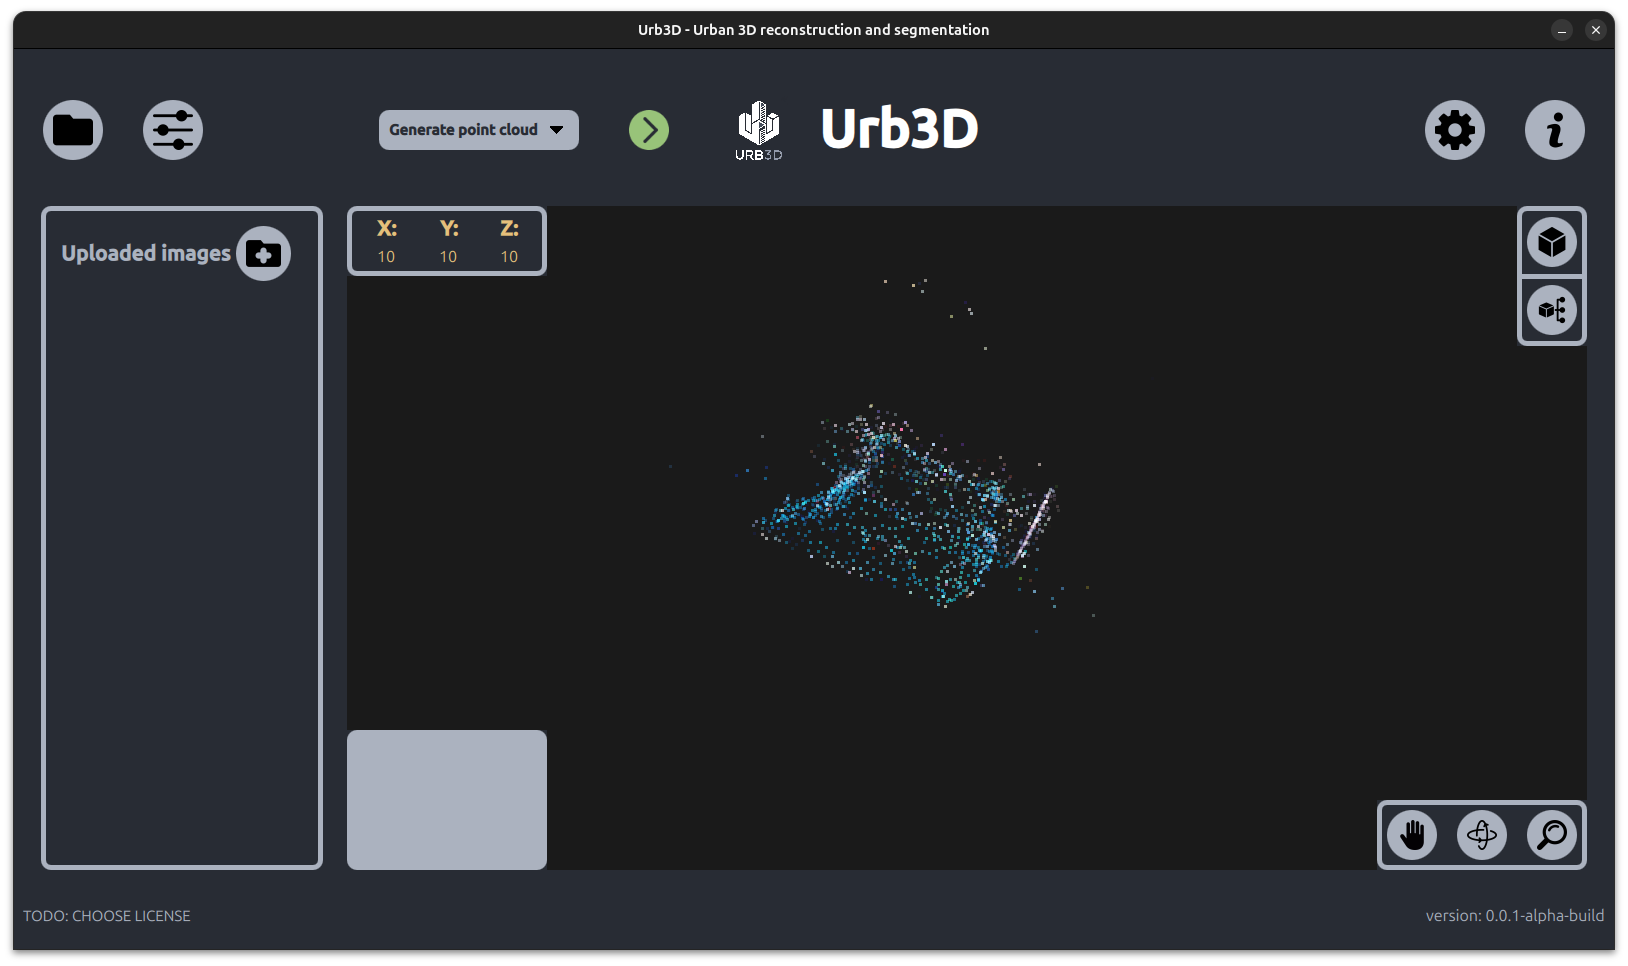
\includegraphics[width=\textwidth]{images/UI-Rendering.png}
    \caption{Zrzut ekranu przedstawiający główny widok aplikacji}
    \label{fig:ui}
\end{figure}

\begin{figure}[!ht]
    \centering
    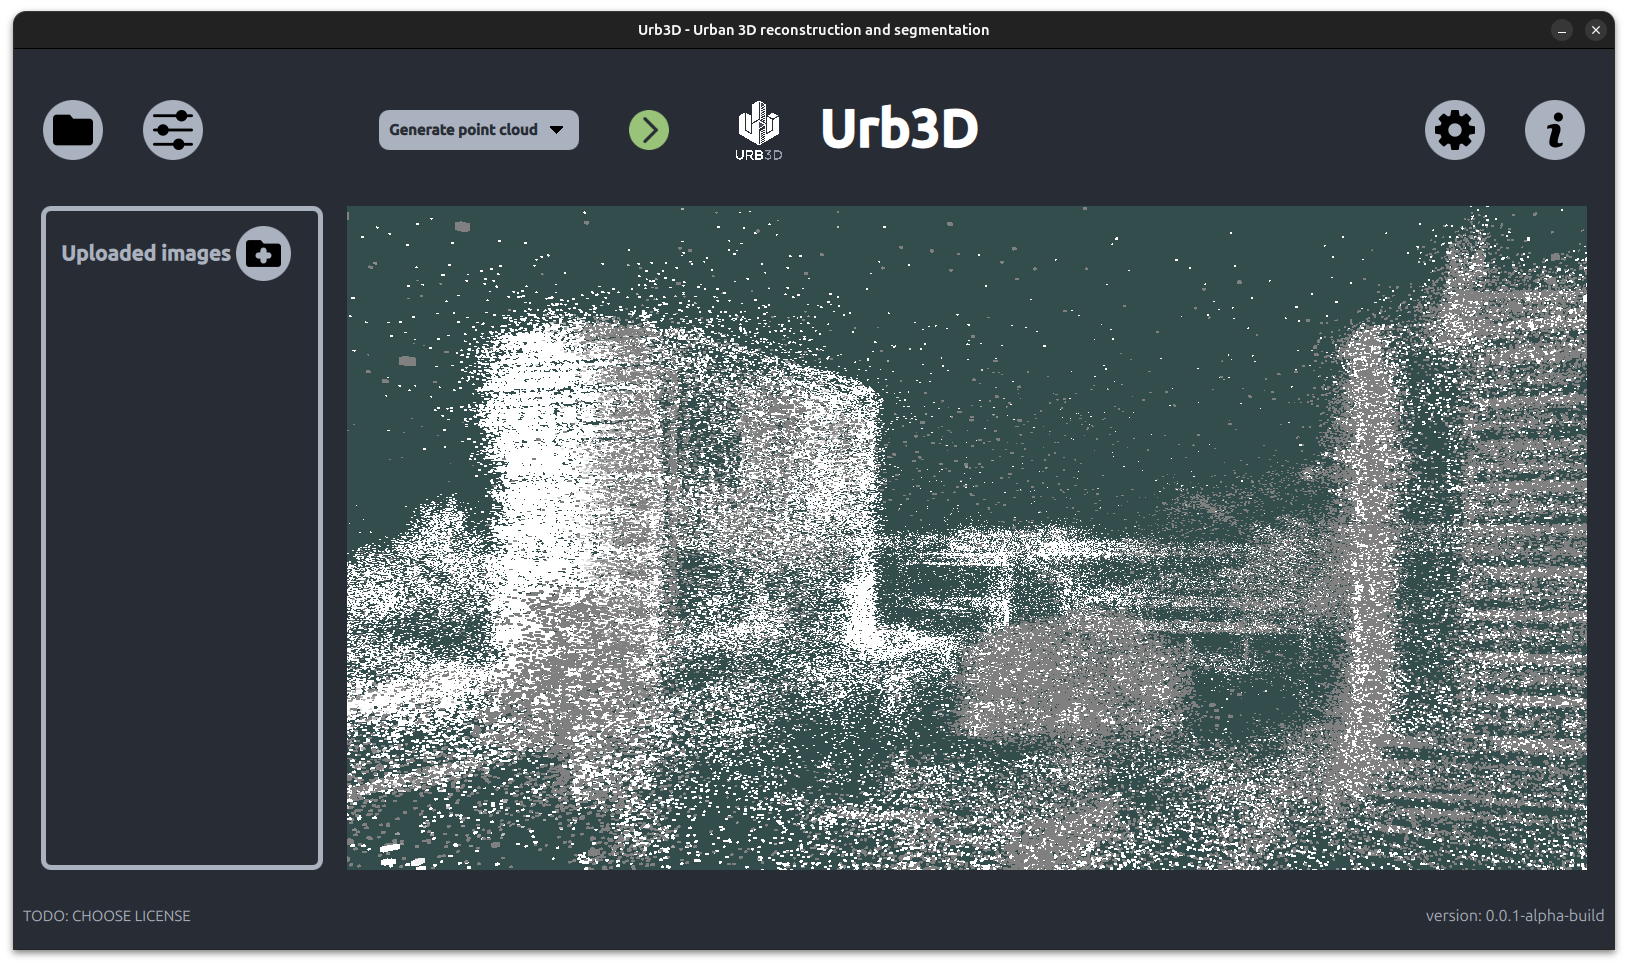
\includegraphics[width=\textwidth]{images/cloud_rendering.png}
    \caption{Zrzut ekranu przedstawiający własny renderer}
    \label{fig:rendering}
\end{figure}

\section{Podsumowanie}





\bibliographystyle{plain}
\bibliography{references}


\end{document}